\documentclass{article}
\usepackage{ctex}
\usepackage{graphicx}
\usepackage{hyperref}
\usepackage{geometry}
\geometry{
    a4paper,
    total={170mm,257mm},
    left=20mm,
    right=20mm,
    top=40mm,
    bottom=35mm
}
\hypersetup{
    colorlinks=true,
    linkcolor=cyan,
    filecolor=cyan,
    urlcolor=blue
}

\title{基于Titanic数据集的决策树算法实践}
\author{王铭嵩}
\date{\today}

\begin{document}
\maketitle
\newpage
\section{数据分析与处理}
数据来源为Kaggle的\href{'https://www.kaggle.com/datasets/vinicius150987/titanic3'}{The Complete Titanic Dataset}数据集。
源文件为一个包含舱位、年龄、性别、是否幸存等信息的csv文件,共有1309条数据。\\
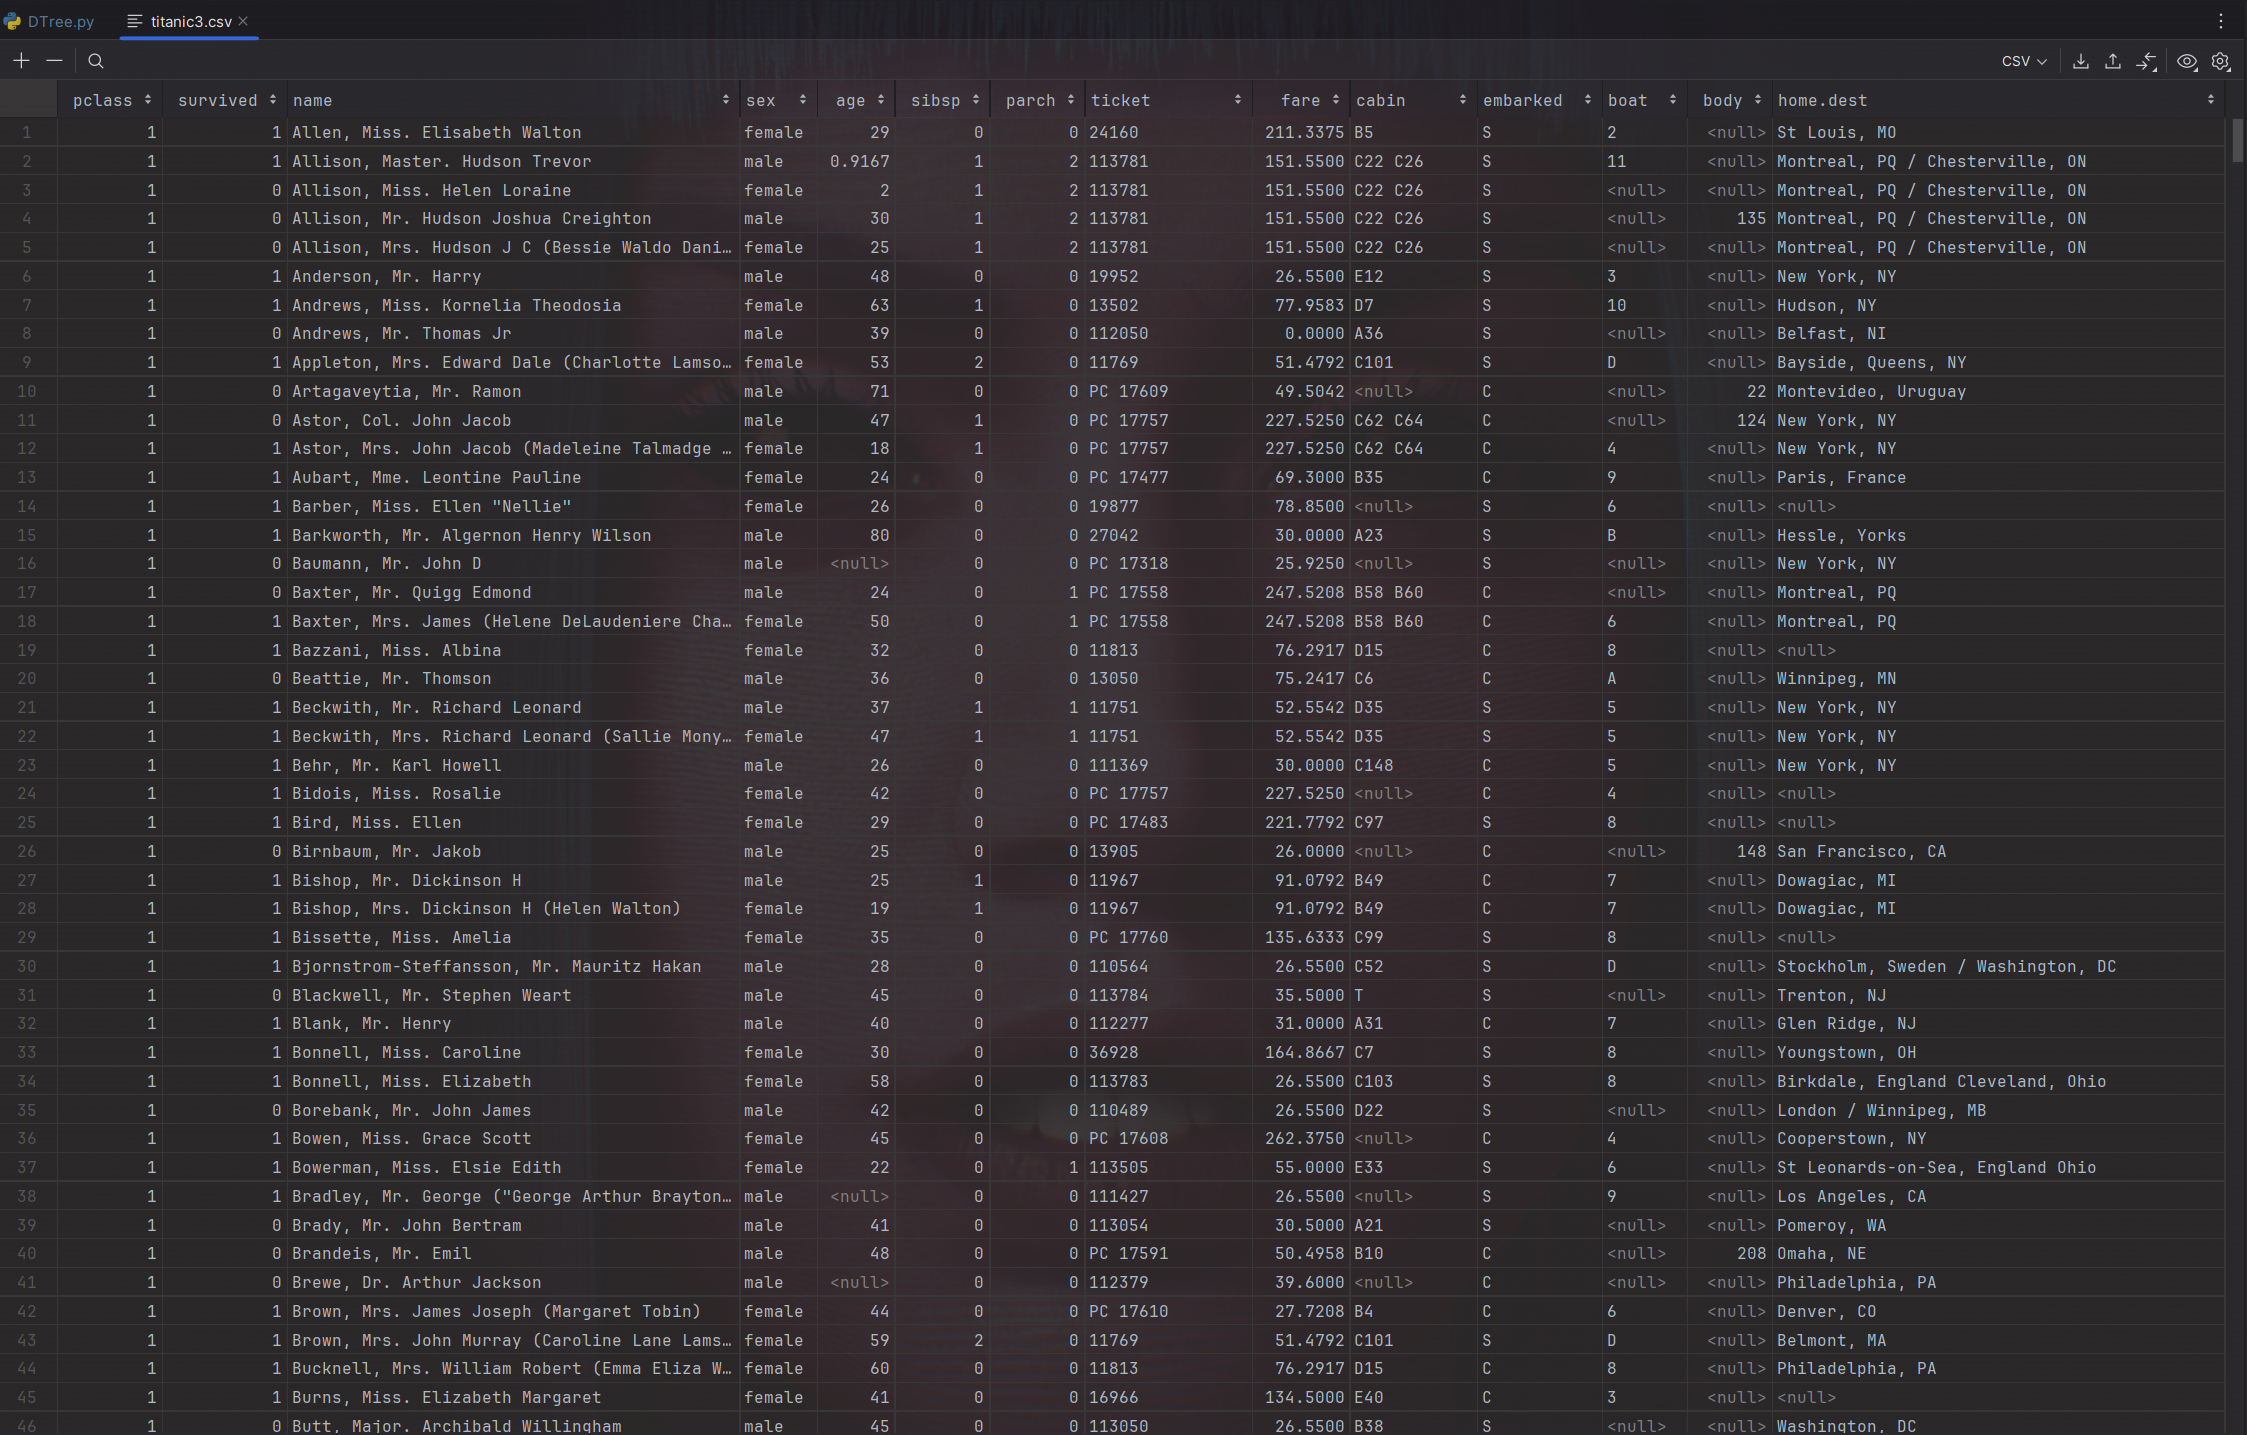
\includegraphics[width=1.0\textwidth]{code_screenshot/datasrc.png}\\
读入数据后清除了年龄、配偶兄弟姐妹数目、父母子女数目信息缺失的条目,并选择舱位、性别、年龄、配偶兄弟姐妹数目、父母子女数目作为特征,是否幸存作为预测目标。\\
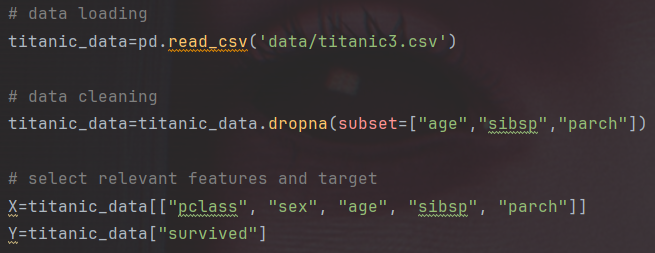
\includegraphics[width=1.0\textwidth]{code_screenshot/dataclean.png}\\
\section{决策树原理与代码}
决策树通过递进的属性判断对样本进行划分,并采用一定的度量标准来决定每一次划分所基于的属性。度量标准一般包括信息增益、信息增益率以及基尼指数,对应ID3决策树,C4.5决策树和CART决策树算法。\\
叶节点采用递归方式生成,达到最大深度或者样本数目小于阈值时停止递归。\\
代码如下,采用scikit-learn库实现。用信息增益作为纯度指标。\\
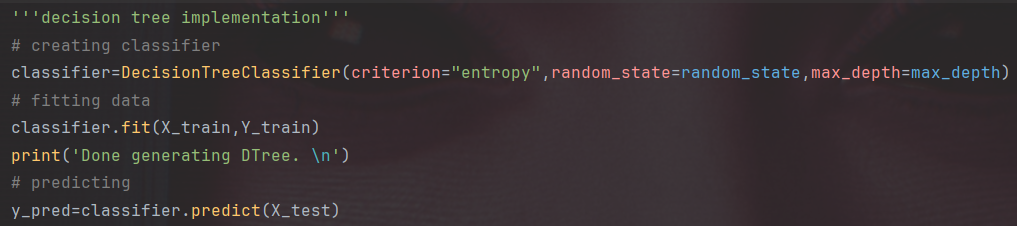
\includegraphics[width=1.0\textwidth]{code_screenshot/DTreeMain.png}\\
\section{验证集评估结果}
分别在最大树高度4到12的情况下对决策树进行评估。验证集为F1-Micro和F1-Macro。以下为各最大树高条件下的各验证集测量值。\\
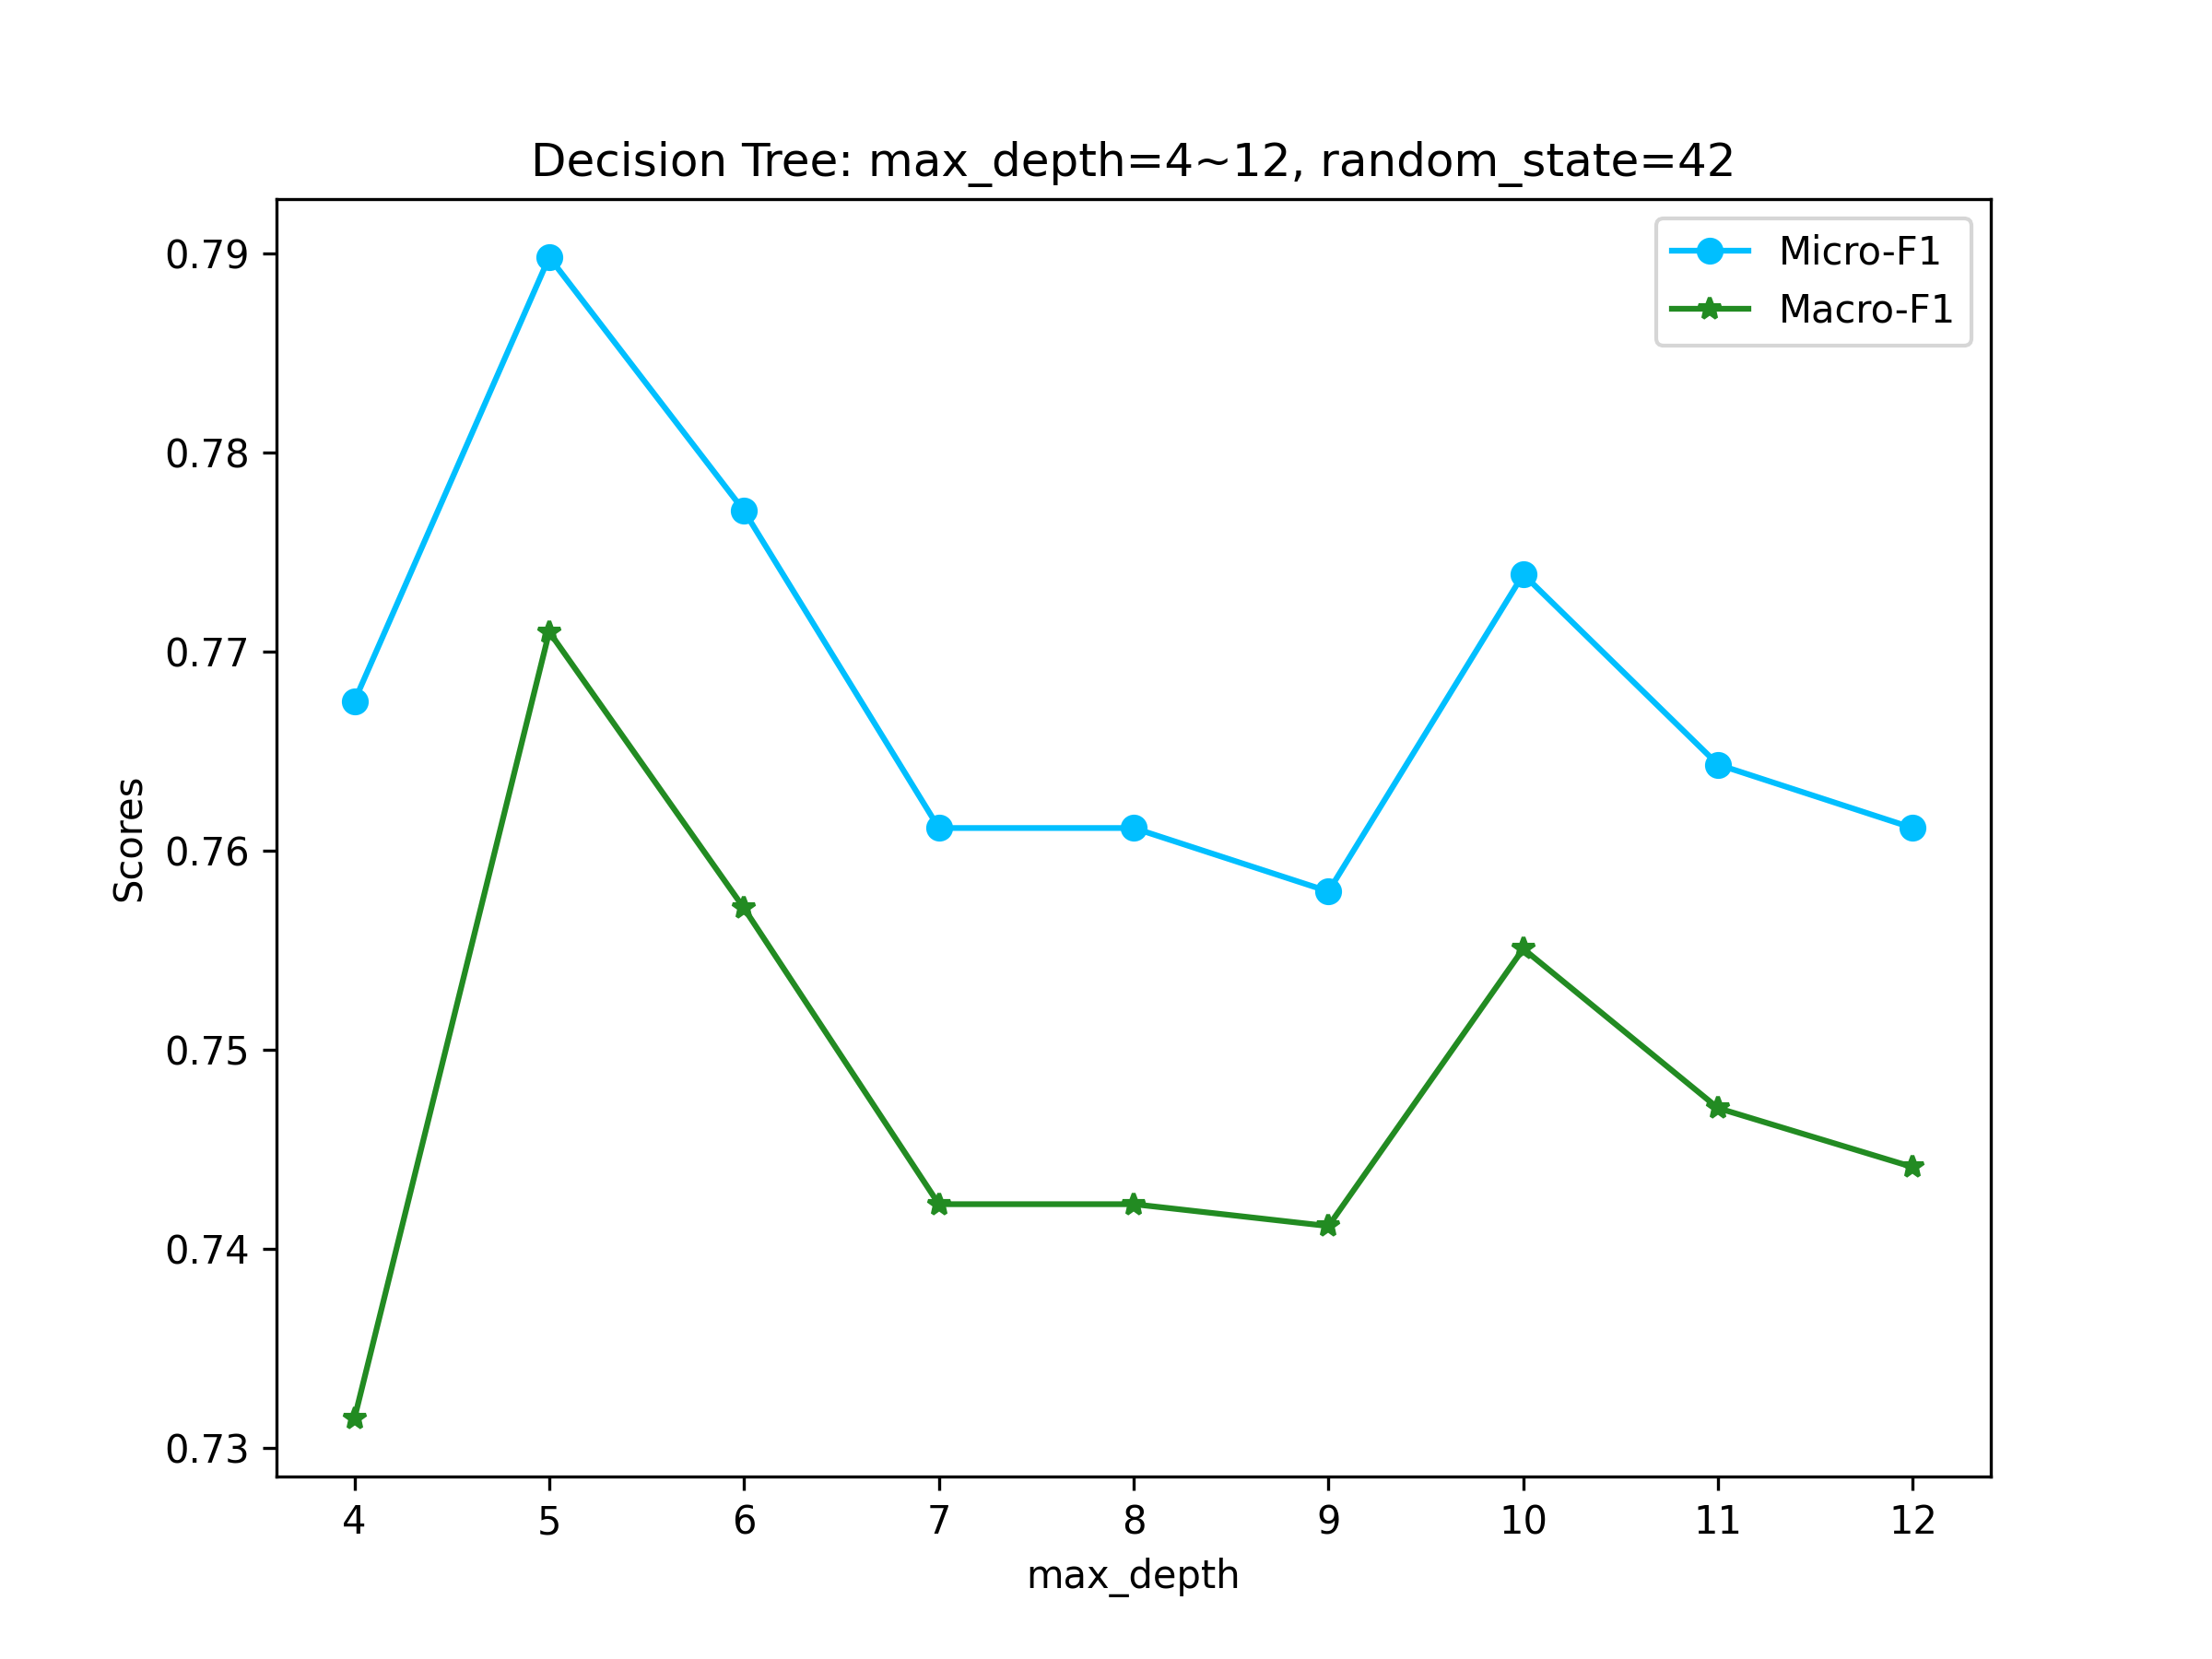
\includegraphics[width=0.85\textwidth]{../python/result/compare_4_to_12.png}\\
\section{决策树可视化}
\subsection{最大树高度为4}
仅显示部分最大树高度下的可视化。完整可视化图片可在\href{'../python/result/'}{../python/result}目录下查看。\\
\includegraphics[width=1.0\textwidth]{../python/result/tree_dep=4_rand=41.png}\\
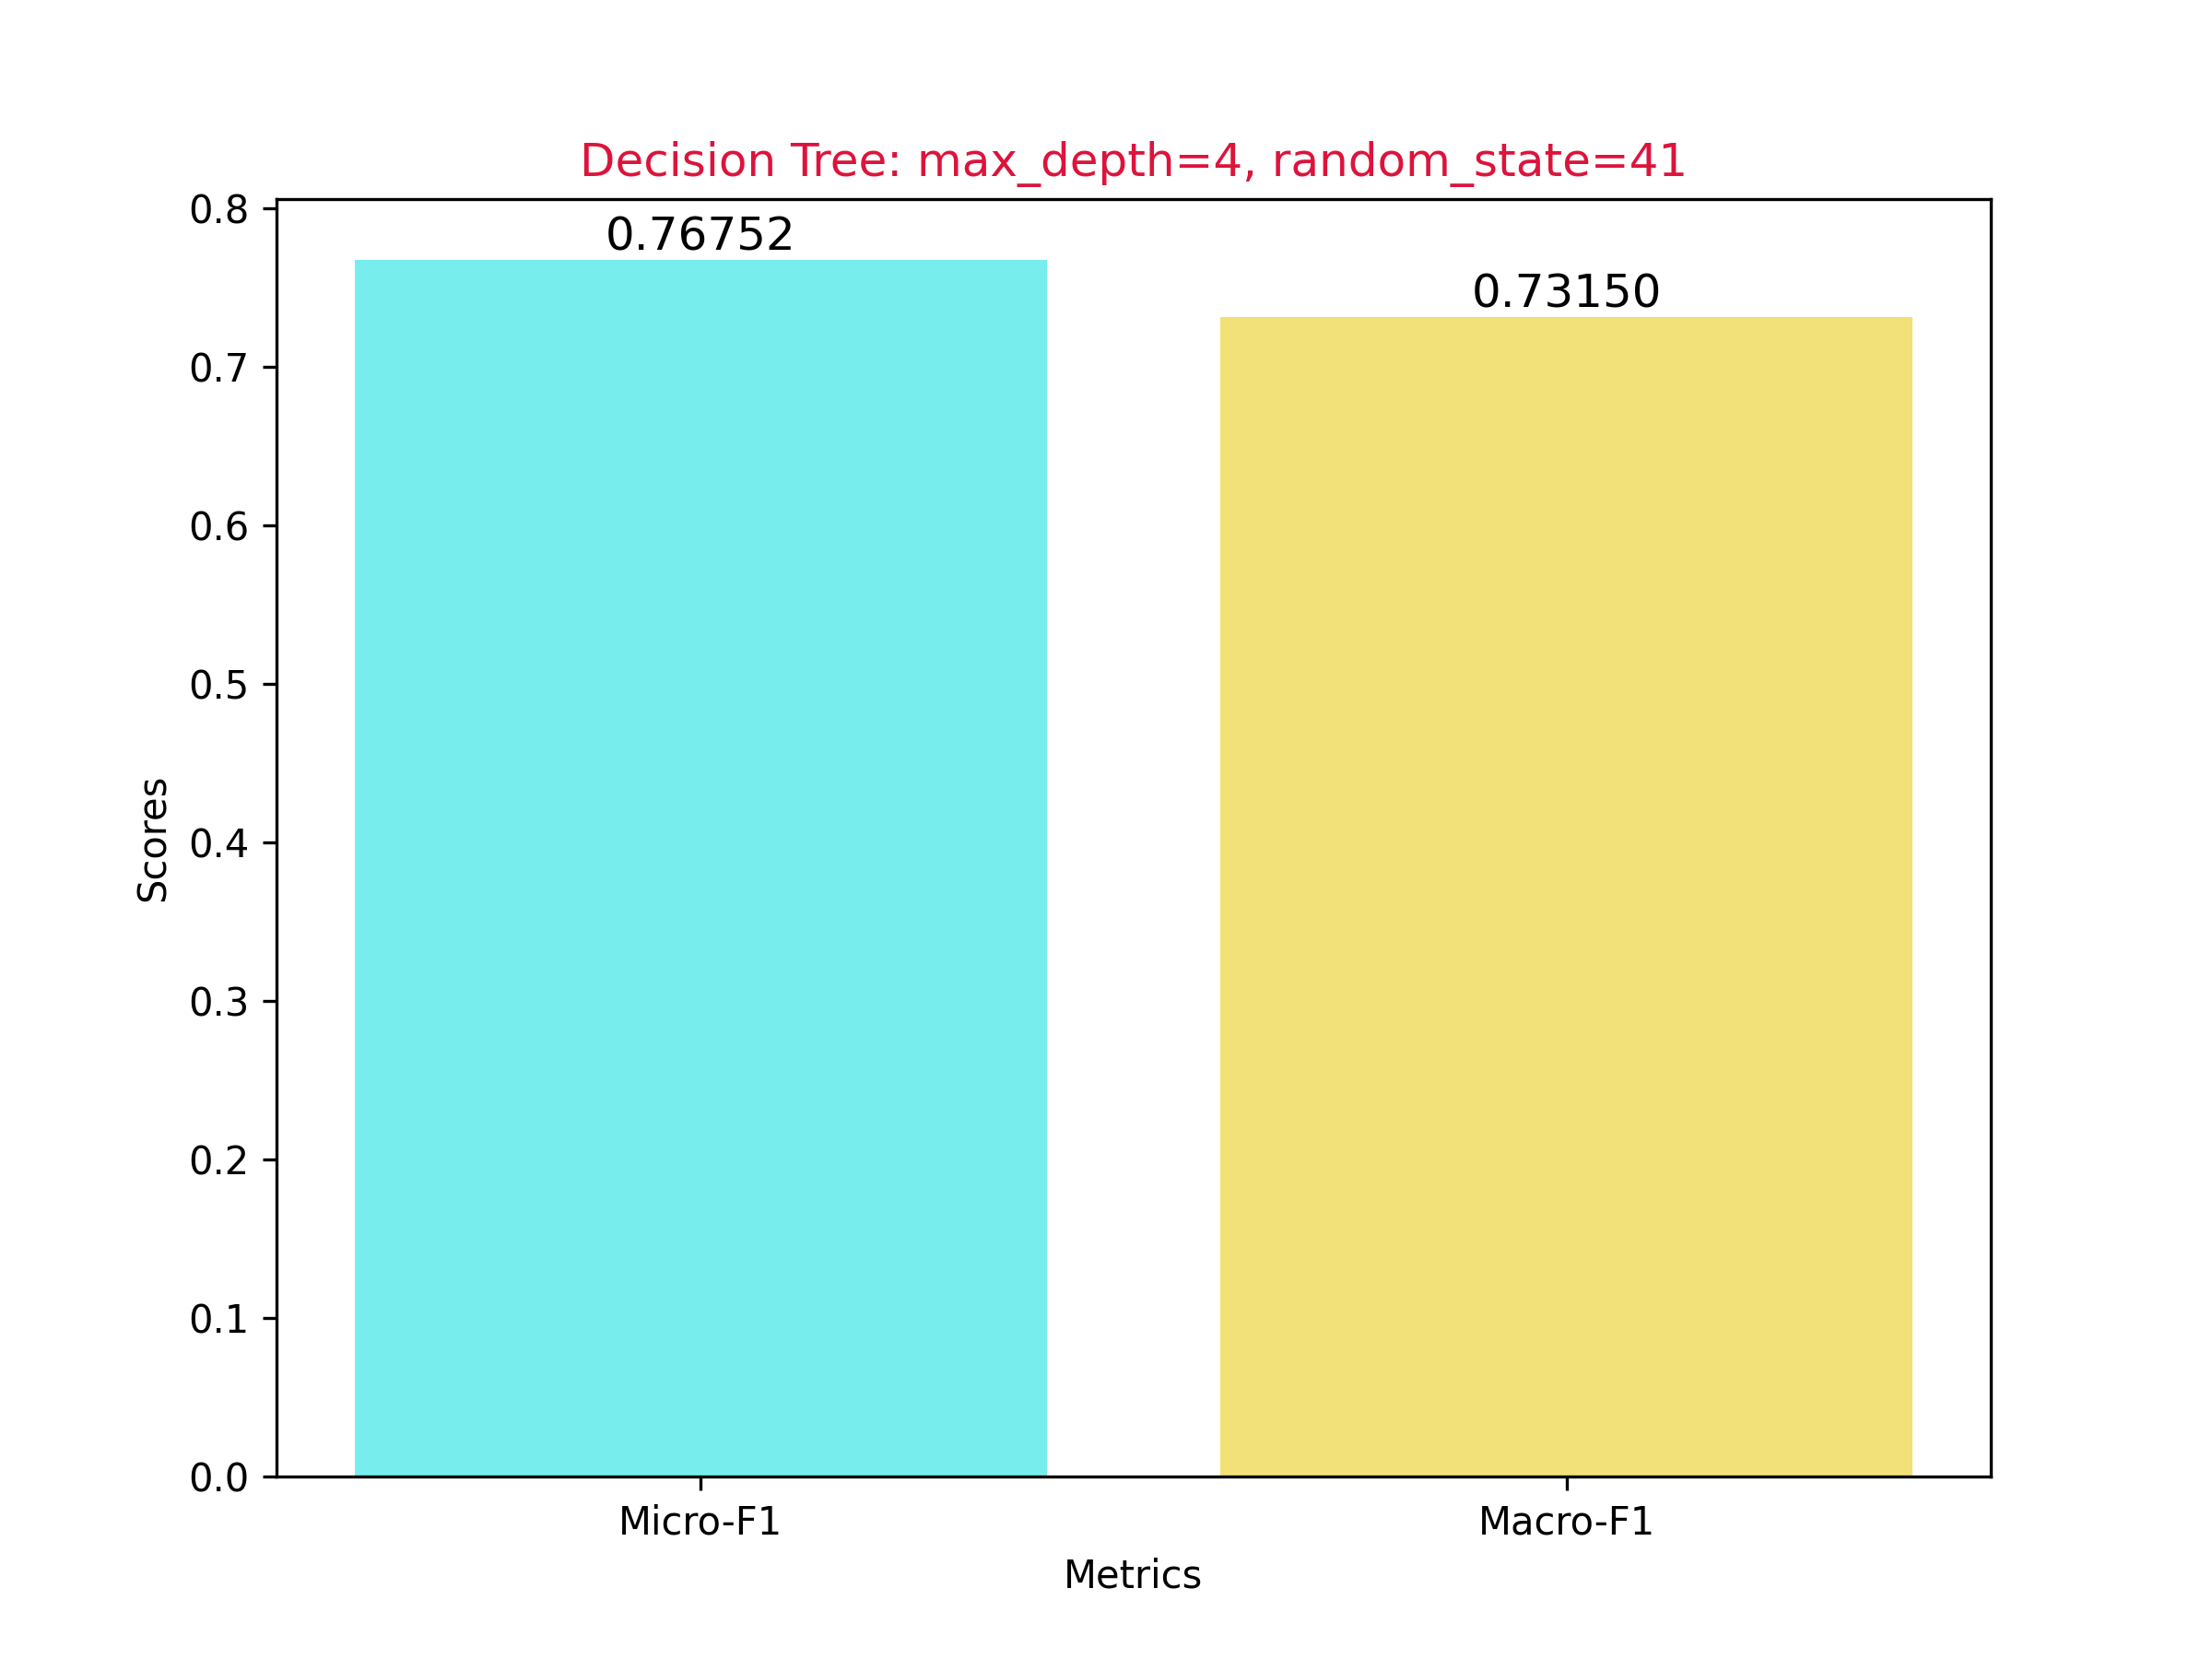
\includegraphics[width=0.7\textwidth]{../python/result/score_dep=4_rand=41.png}\\
\subsection{最大树高度为9}
\includegraphics[width=1.0\textwidth]{../python/result/tree_dep=9_rand=41.png}\\
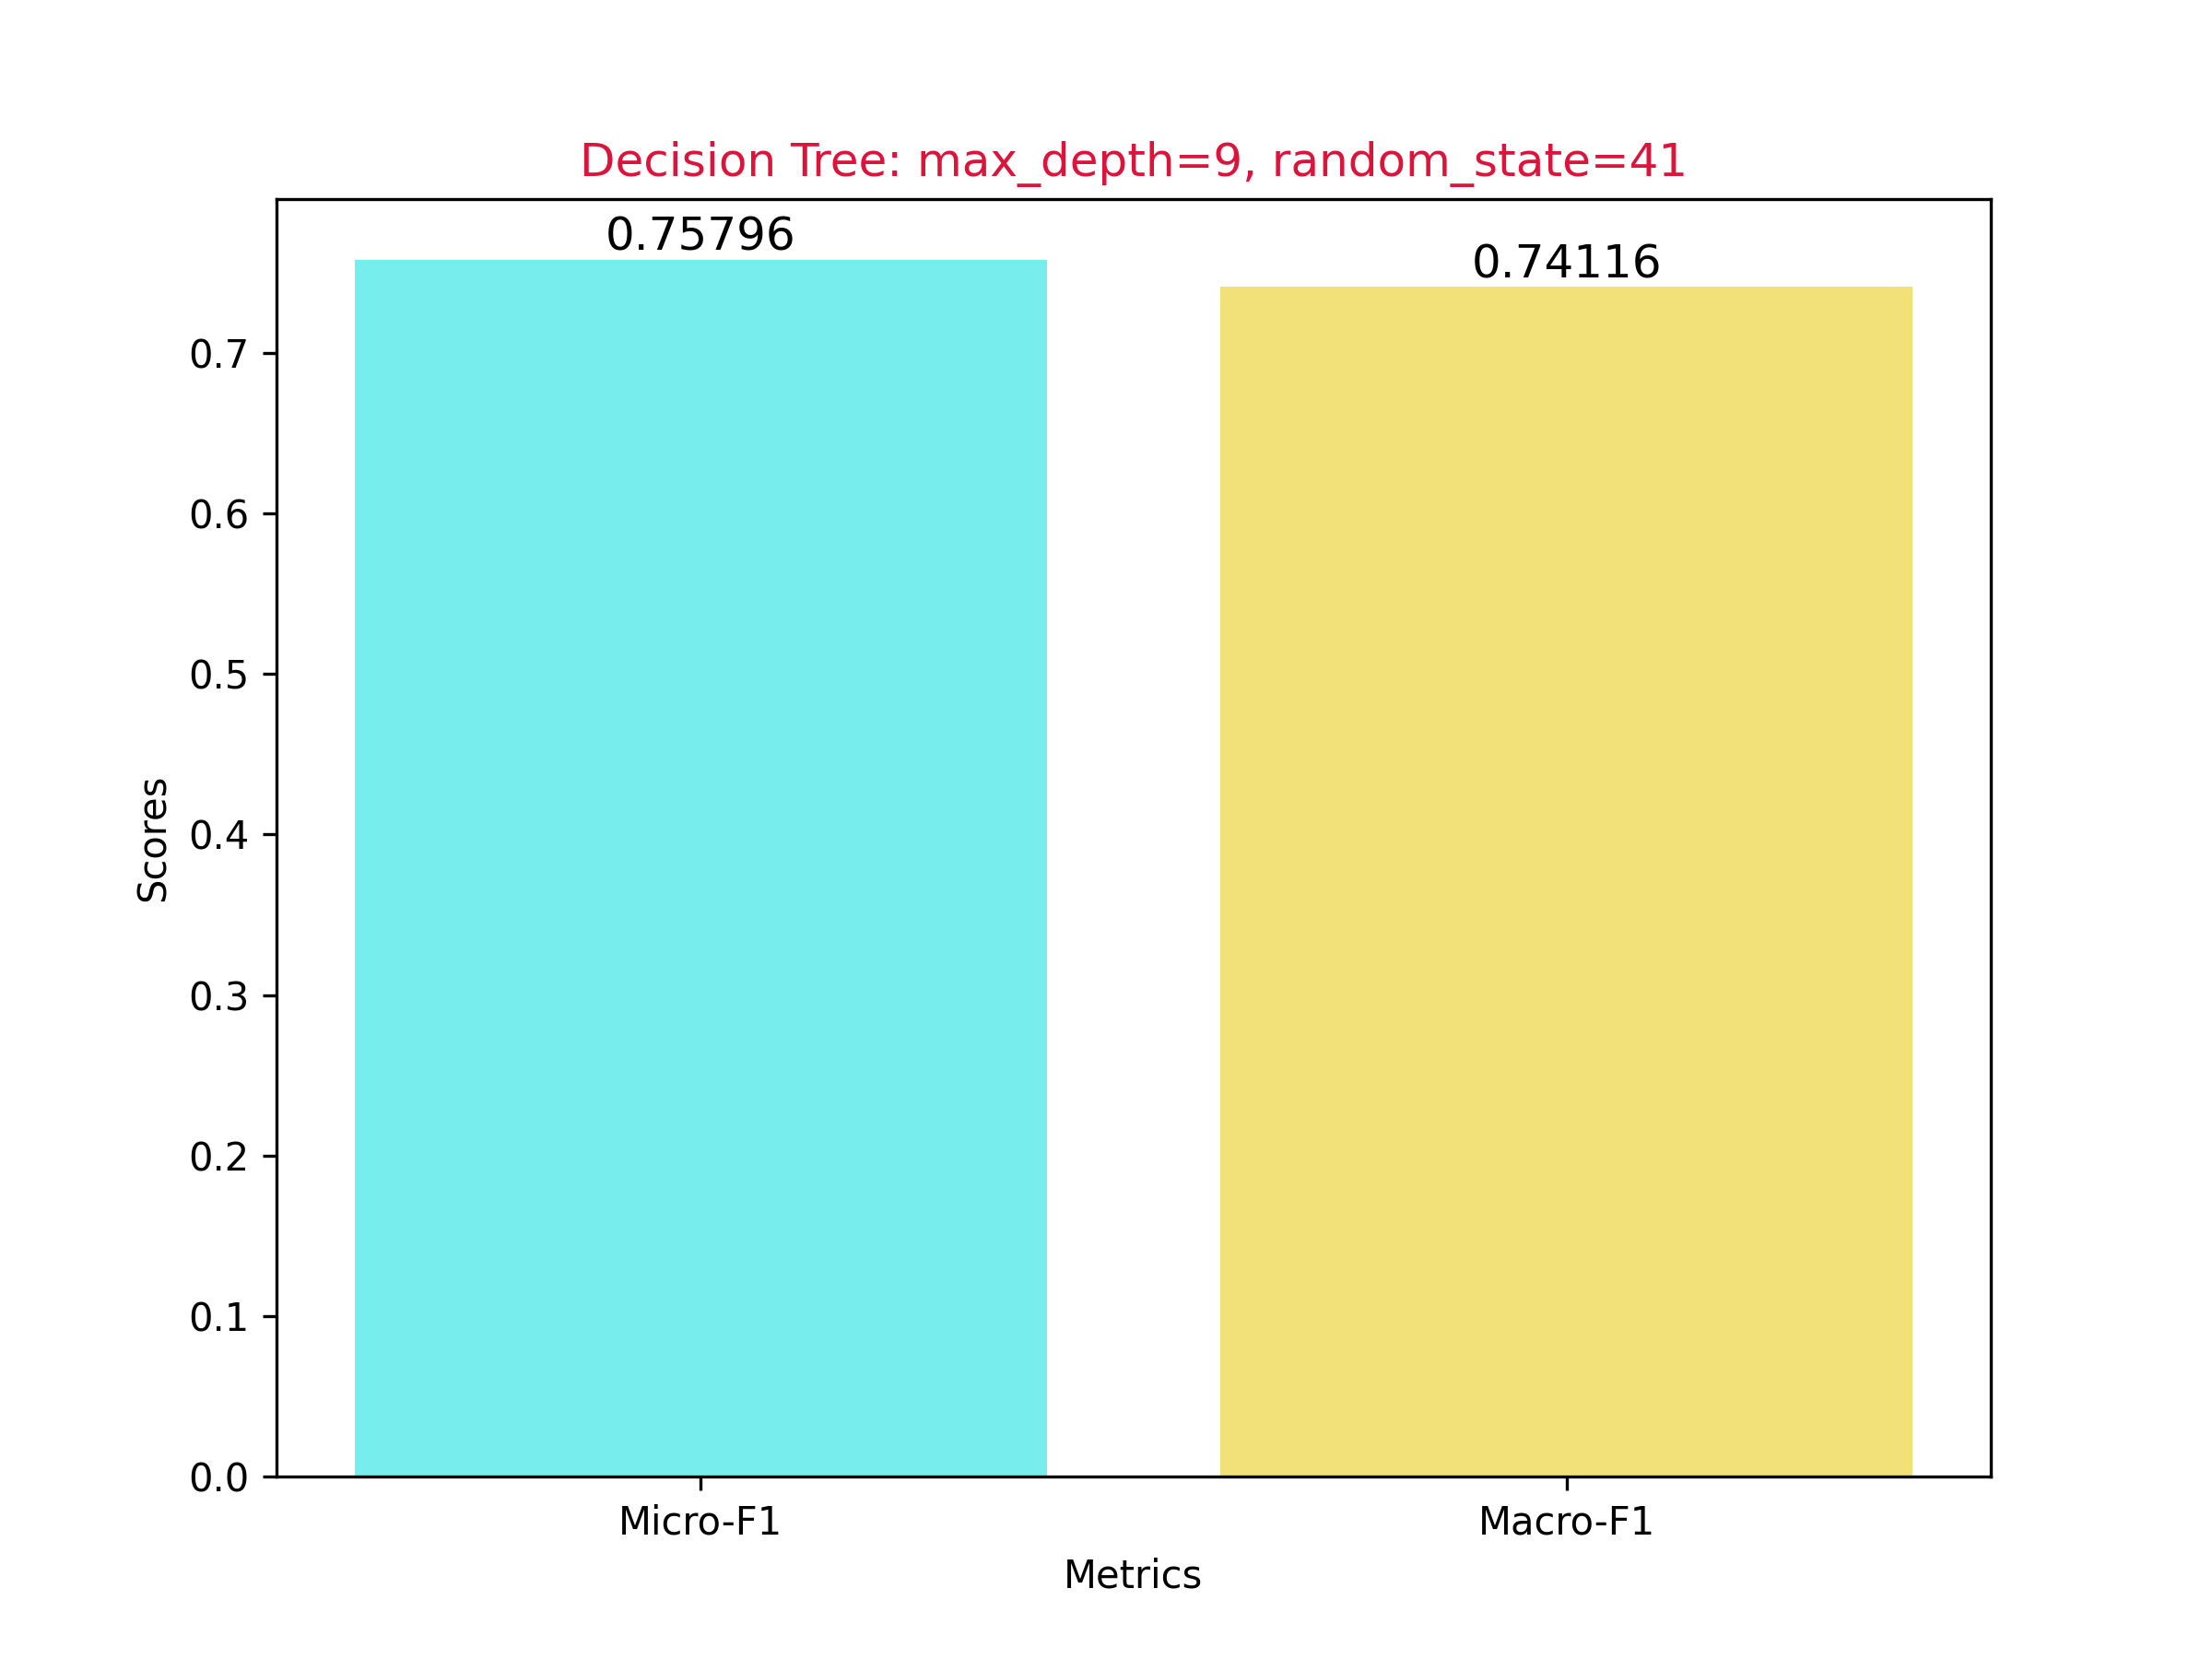
\includegraphics[width=0.7\textwidth]{../python/result/score_dep=9_rand=41.png}\\
\subsection{最大树高度为12}
\includegraphics[width=1.0\textwidth]{../python/result/tree_dep=12_rand=41.png}\\
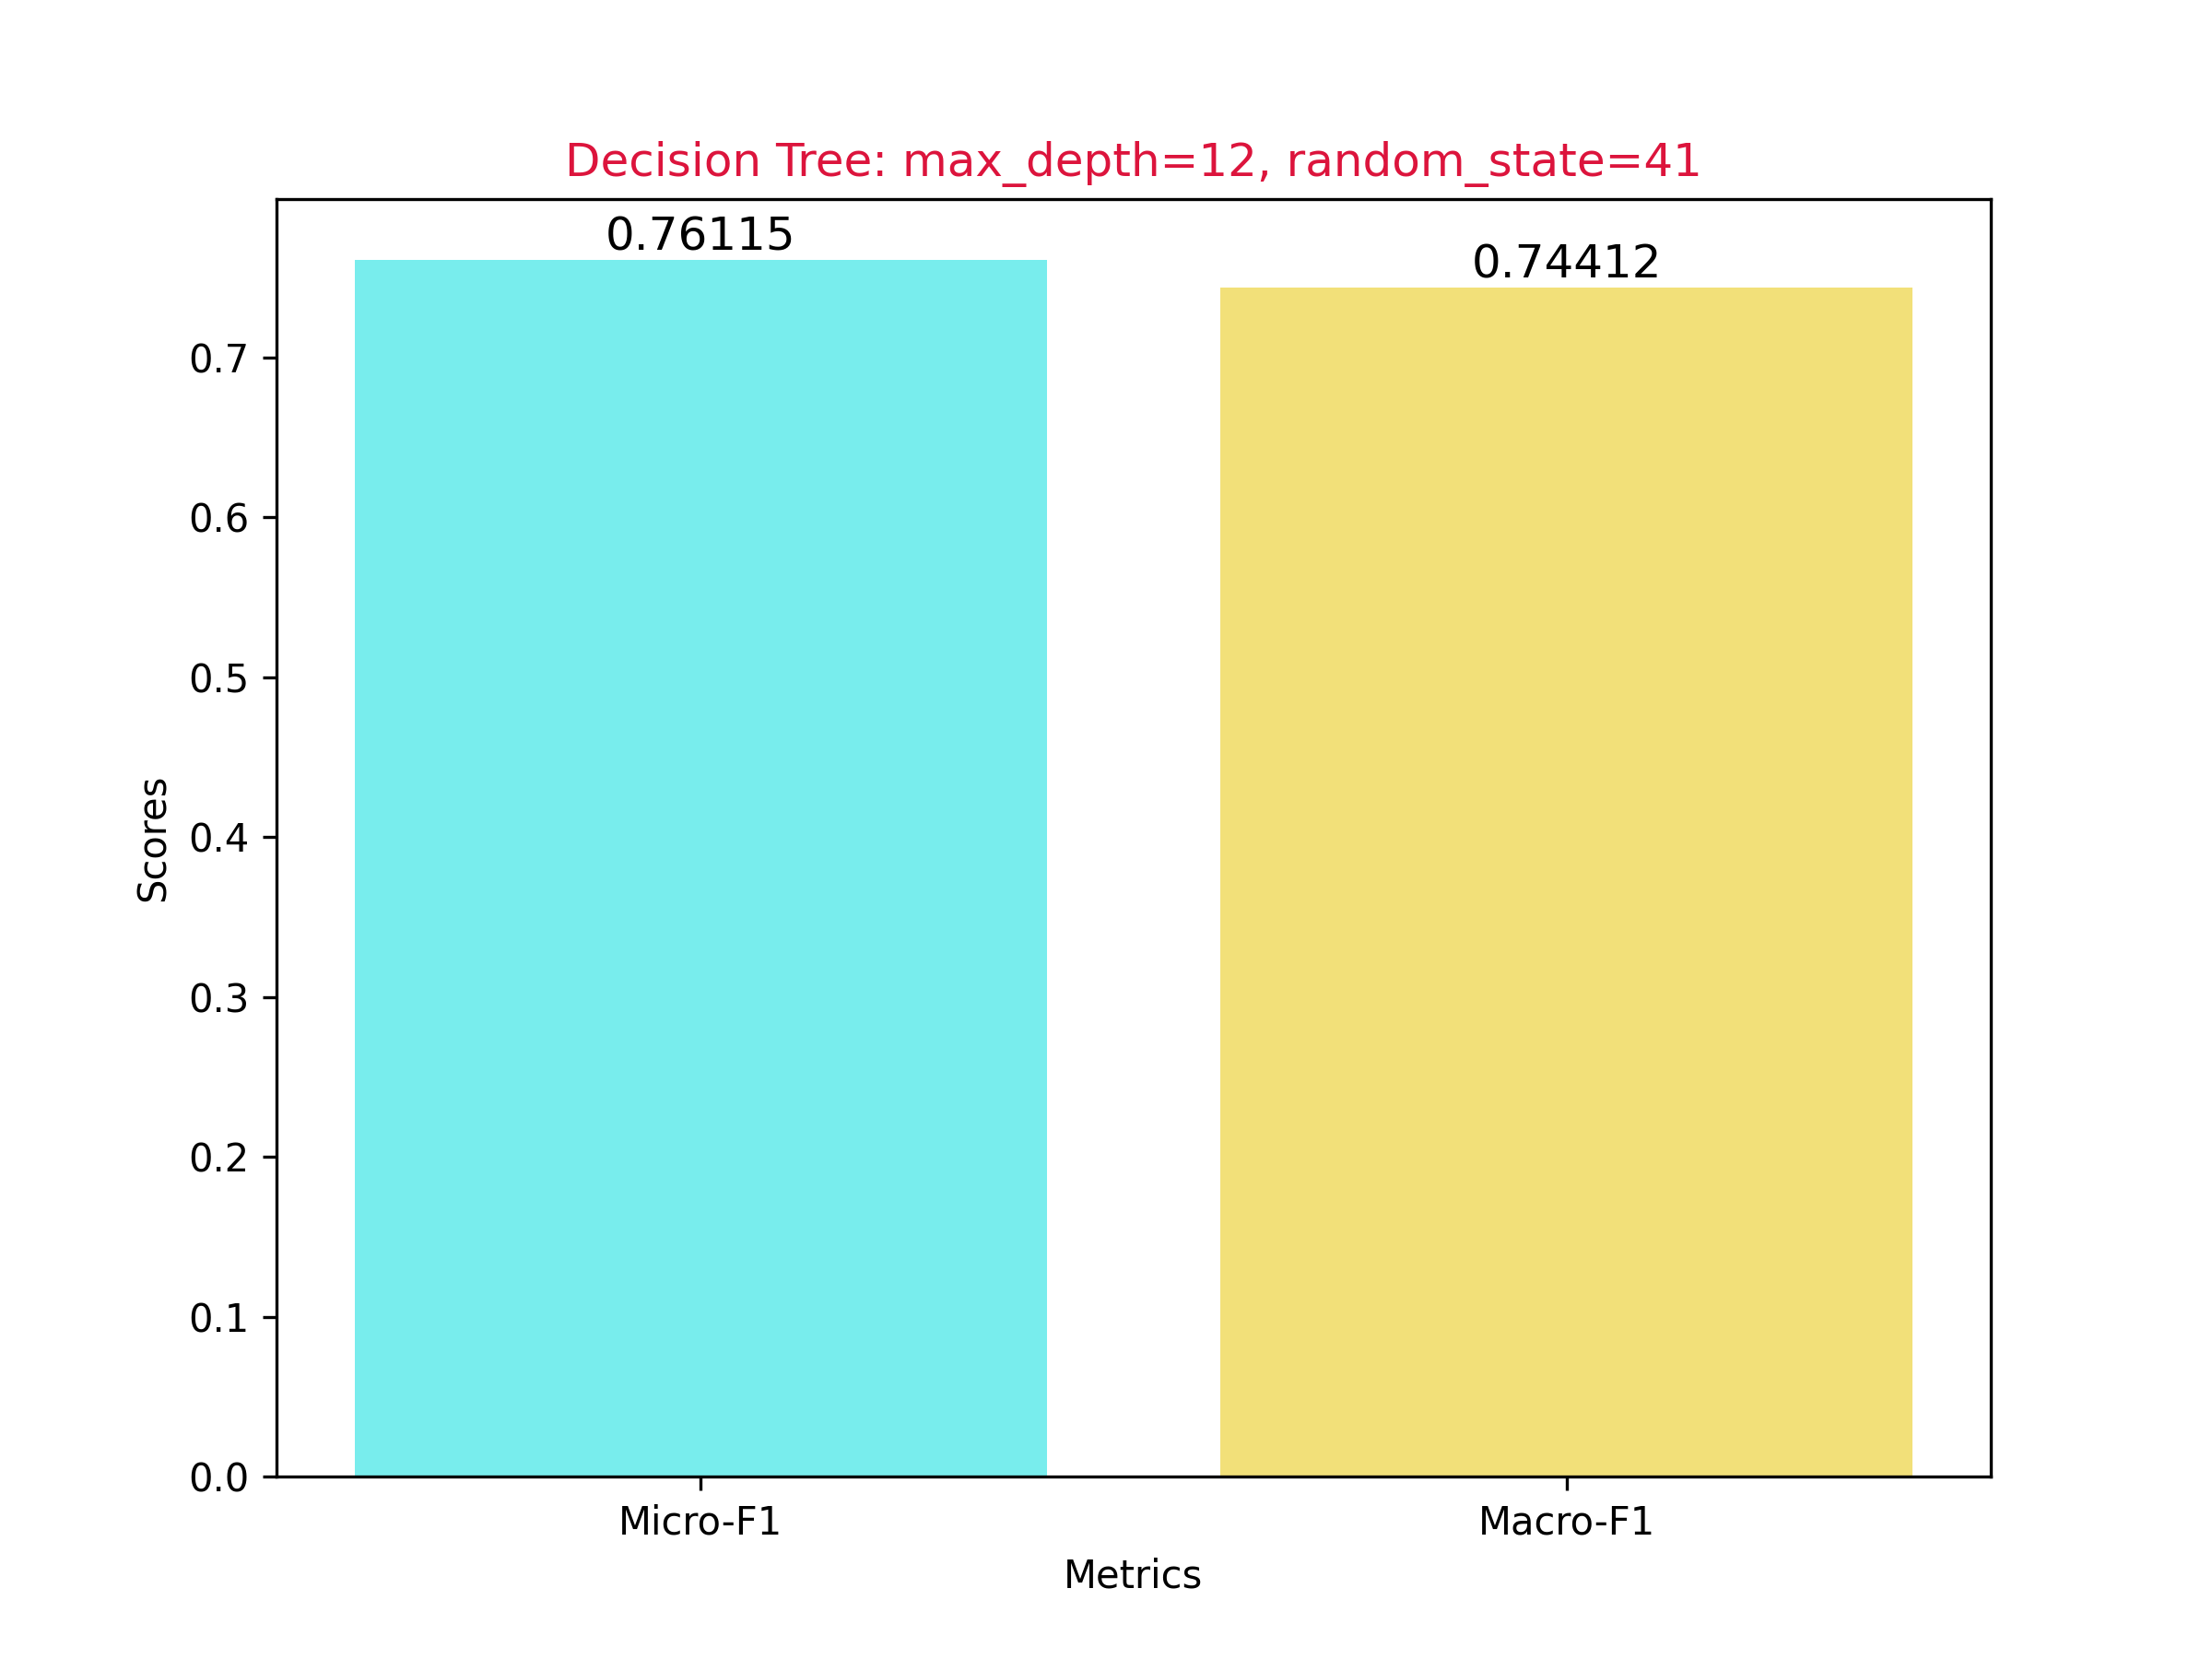
\includegraphics[width=0.7\textwidth]{../python/result/score_dep=12_rand=41.png}\\

\end{document}
